% This is a LaTeX input file.

\documentclass[twoside,11pt]{article}
\usepackage{tabularx}
\usepackage{fancyhdr}
\usepackage{listings}
\lstset{language=Java, basicstyle=\small, frame=lines, stringstyle=\color[RGB]{42,0,255}\ttfamily,
identifierstyle=, keywordstyle=\color[RGB]{127,0,85}\bfseries, commentstyle=\color[RGB]{63,127,95}}

\usepackage{color}
\usepackage{float,graphicx}
\restylefloat{figure}
\usepackage[format=hang,margin=10pt]{caption}

\setlength{\headheight}{14.0pt}
\setlength{\textwidth}{6in}
\setlength{\textheight}{8.5in}
\setlength{\oddsidemargin}{0in}
\setlength{\evensidemargin}{0in}
\setlength{\topmargin}{0in}
\setlength{\footskip}{0.75in}

\newcommand{\bold}[1]{\textbf{#1}}
\newcommand{\rt}[1]{{\color[RGB]{237,24,30}{#1}}}
\newcommand{\gt}[1]{{\color[RGB]{47,139,32}{#1}}}
\newcommand{\yt}[1]{{\color[RGB]{255,210,60}{#1}}}
\newcommand{\PAA}{Appearance Agent\space}


\begin{document}


\title{\emph{\textbf{Appearance Agent}\\
Design Specification}}
\author{Marden P. Marshall}
\date{Release 0.5\\
July 28$^{th}$, 2007}

\maketitle

\begin{figure}[ht] \centering
\scalebox{0.35}{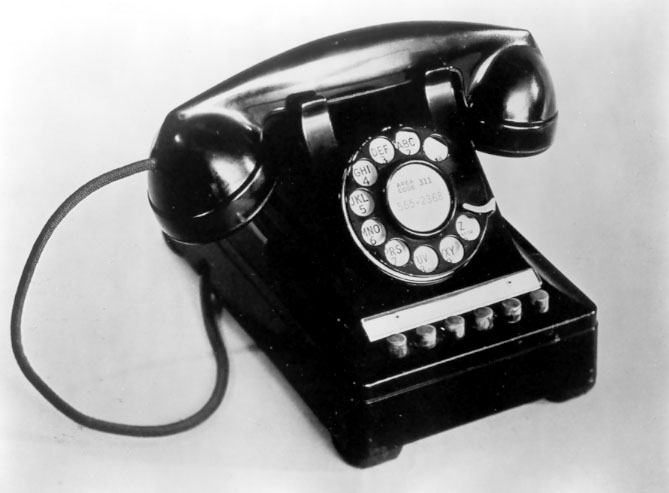
\includegraphics{keyset.jpg}}
\end{figure}

\thispagestyle{empty}
\clearpage
\thispagestyle{empty}
\begin{center}
\textbf{Change Log}

\begin{table}[h]
\begin{center}
\newcolumntype{C}{>{\centering\arraybackslash}X}
\begin{tabularx}{\linewidth}{
|>{\setlength{\hsize}{.4\hsize}}C
|>{\setlength{\hsize}{.6\hsize}}X
|>{\setlength{\hsize}{2.0\hsize}}X|} \hline
\textbf{Version} & \textbf{\centerline{Date}} & \textbf{\centerline{Changes}}  \\
\hline \hline
0.1 & July 5$^{th}$, 2007 & Initial internal release. \\
\hline
0.2 & July 6$^{th}$, 2007 & Minor typographical error corrections and cosmetic
improvements. \\
\hline
0.3 & July 15$^{th}$, 2007 & Initial public release following internal review. \\
\hline
0.4 & July 17$^{th}$, 2007 & Clarification of Appearance Number Allocation and
initial description of Appearance State Publisher component. \\
\hline
0.5 & July 28$^{th}$, 2007 & Updated copyright notice. Updated Dependency
Injection section (Now using Guice). \\
\hline
\end{tabularx}
\end{center}
\end{table}

\end{center}
\clearpage

\pagestyle{fancy}
\fancyhead{}
\fancyhead[LO,RE]{Appearance Agent - Design Specification}
\fancyhead[RO,LE]{\thepage}
\fancyfoot{}
\fancyfoot[C]{Copyright \copyright \hspace{1pt} 2007 Bluesocket Corporation}
\renewcommand{\footrulewidth}{0.4pt}
\pagenumbering{roman}

\tableofcontents
\clearpage
\listoffigures
\lstlistoflistings
\clearpage

\pagestyle{fancy}
\fancyhead{}
\fancyhead[LO,RE]{Appearance Agent - Design Specification}
\fancyhead[RO,LE]{\thepage}
\fancyfoot{}
\fancyfoot[C]{Copyright \copyright \hspace{1pt} 2007 Bluesocket Corporation}
\renewcommand{\footrulewidth}{0.4pt}

%\setlength{\parskip}{4pt}
\pagenumbering{arabic}

\section{Introduction}
The fundamental purpose of the \PAA is to provide a centralized repository for the collection and
publishing of dialog state information. Various extensions of this core functionality can be added
in order to support various business class telephony features, most notably Bridged Line Appearance
(BLA) and Busy Lamp Field (BLF). Other services that can leverage state information published by the
\PAA might be, for example, an Attendant Console or a Call Pickup service.

\subsection{Design and Development Process}
This project is being undertaken within an Agile process.  As a result, this document will initially
begin describing the design at a high level.  As the project progresses, this document will evolve
with the level of detail progressively increasing. As each sprint is completed, the document will be
updated to reflect the actual design which was employed.

\subsection{Implementation Phases}
In order to meet market timing demands, the \PAA will be developed in phases:
\begin{itemize}
  \item{\bold{Phase 1}}
  \begin{itemize}
    \item Core \PAA functionality
    \begin{itemize}
      \item Dialog Info Package
      \item Subscription Client
      \item Subscription Server
      \item Subscription Management
      \item Dependency Injector
    \end{itemize}
    \item BLA feature
    \item Appearance state publishing
    \item 500 Appearance capacity
  \end{itemize}
  
  \item{\bold{Phase 2}}
  \begin{itemize}
    \item Centralized BLA line allocation
    \item Appearance state publishing via JMS
    \item BLF feature
    \item 2500 Appearance capacity
  \end{itemize}
  
  \item{\bold{Phase 3}}
  \begin{itemize}
    \item Clustering
    \item High Availability
    \item 5000 Appearance capacity
  \end{itemize}
\end{itemize}

\section{Key Design Issues}
There are several key design issues which must be given particular attention to detail as they are
critical for the overall success of this project. These are:
\begin{itemize}
  \item Subscription Management
  \item XML Data Binding
  \item Signaling Over Reliable Transport
  \item SIP Stack Performance
\end{itemize}
  
\subsection{Subscription Management}
  The \PAA will be subjected to a high degree of signaling traffic.  A large
  percentage of this traffic will be for the purpose of either creating,
  servicing or renewing dialog subscriptions.  The worst case scenario would
  most likely be with shared line appearances.  Here, each appearance would
  be associated with two subscriptions, one originating from the \PAA and one
  terminated at the \PAA.  At a maximum configuration of 5000 appearances, that
  would represent 10,000 subscriptions.  With a worst case subscription
  subscription period of five minutes, that would translate to slightly more
  than 33 subscription renewals per second.  This is believed to be a sustainable rate,
  assuming that the traffic rate remains flat.

  With such high data rates, any type of sustained burst or clumping of subscription traffic would
  quickly result in the server becoming congested. It is also very likely that the server would not
  be able to ever recover from this condition, resulting in a catastrophic failure.  To help avoid
  this scenario, it will be necessary for the server to shape the subscription traffic by schedule
  the subscriptions evenly over time.  This will be necessary both for subscriptions that are
  initiated by the server as well as subscriptions being accepted by the server.
  
\subsection{XML Data Binding}
  Given that the majority of the data that is either generated by or processed by the \PAA is XML,
  it is critical that a fast, efficient and reliable XML data binding framework be employed.  With
  there, for example, being a one-to-one correlation between marshaling / unmarshaling operations
  and subscription renewals, the performance of these operations is crucial. Also of importance is a
  sensible data model. This is necessary both for minimizing memory footprint and the clarity and
  maintainability of the surrounding software.
  
\subsection{Signaling Over Reliable Transport}
  Many of the telephony features that the \PAA will either directly or indirectly support are
  customer facing.  As such, failures resulting in such misbehavior's as stuck line status lamps or
  the inability to pick up a call result in high levels of customer dissatisfaction.
  
  The signaling traffic that occurs between the stations and the \PAA is both high in frequency and
  large in size.  Packet size can easily exceed the networks physical layer MTU.  When running over
  a UDP transport, this would then result in IP fragmentation.  Given the unreliability of IP
  fragment reassembly, this could result in either dropped packets or truncated signaling messages. 
  Experiments have shown that some user agents fail to always indicate to the far end when a
  truncated messages has been received.  This can result in annoying failures that are also very
  difficult to diagnose.
  
  The best solution to this problem is to run the signaling over a reliable transport such as either
  TCP or TLS.  It will not completely prevent the case of lost packets, but the guaranteed
  reliability of TCP/TLS segmentation/reassembly should completely eliminate truncated packets.
  Utilizing a connection oriented transport can also result in a significant performance improvement
  with the underlying SIP stack.  Also, due to the added reliability, it will allow for the use of a
  much longer subscription period in the range of 30 to 60 minutes.
  
\subsection{SIP Stack Performance}
  The SIP stack is most likely the second most critical component in terms of performance and
  reliability, with the XML Data Binding component being first.  The stack must be able to sustain a
  rate of 50 or more transactions per second while still leaving sufficient CPU and memory resources
  for the remaining functionality.  Given the potentially large number of concurrent SIP sessions,
  it is also important that the stack do a good job at managing system resources such as memory and
  threads.


\section{Design Details}
Figure \ref{AABlockDiagram} shows a high level software block diagram of the \PAA. Working in a
bottom-up approach, this section will cover the functional breakdown and design of each block.

\begin{figure}[ht] \centering
\scalebox{0.75}{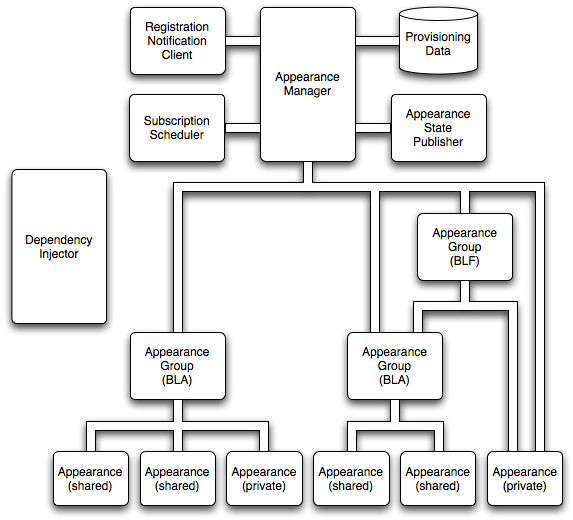
\includegraphics{AABlockDiagram.jpg}}
\caption{Appearance Agent Block Diagram}
\label{AABlockDiagram}
\end{figure}

\subsection{Appearance}
The Appearance component is a logical representation of an actual user agent appearance, typically a
``line'' on a phone.  When instantiated, an Appearance instance will be associated with a specific
registered contact within the PBX domain.  From there, the primary role of the Appearance is to
collect, in near real time, the dialog states of the associated UA appearance. The collected dialog
states are then made available to other components of the \PAA.

\subsubsection{Appearance Sub-types}
There are different sub-types of the Appearance component.  Which sub-type actually is instantiated
depends upon what the target UA's appearance type is and what it's capabilities are.  In theory it
could be possible to determine programmatically, but instead, this will be a provisioned attribute. 
These are the currently planned sub-types:

\begin{itemize}
  \item \bold{Shared}

  Dialog states are collected from the target appearance by subscribing for \bold{dialog;ma} events.
   The target appearance must therefore support and be provisioned as a ``shared'' line.

  \item \bold{Private}

  Dialog states are collected from the target appearance by subscribing for \bold{dialog} events.

  \item \bold{Simulated}

  Dialog states are derived from information received from the proxy components of the PBX as well
  as by directly subscribing to the appearance, if supported.  This allows, at a minimum, the
  ability to maintain dialog states for UA's which do not support direct publishing of such and in
  the case where the UA does support some form of dialog state publishing, the ability to cross
  check the information.
\end{itemize}

\subsubsection{Subscription Client}
In order to collect the required dialog state information in a near real time fashion, the
Appearance will maintain a Subscription Client.  The specific mode that the client will operate
depends upon the specific sub-type of the Appearance.  The Subscription Client is passive in that it
is scheduled and driven by the Subscription Scheduler component.

Note: \emph{The Subscription Client is expected to be able to subscribe directly to the associated
appearances contact of registration.  The Registrar, via its subscription notification events, must
supply this level of detail.  Forking of subscribe requests are not supported.}

\subsubsection{Dialog Info Package}
Critical to the Appearance component and the Subscription Client is the Dialog Info Package.  This
provides a data mapping to the dialog-info XML document as per RFC4235.  Marshaling and unmarshaling
is provided by the JiBX XML data binding framework.  By using this form of data binding, the same
run-time representation of appearances dialog state information is also used in the processing and
publishing of dialog-info payloads. Figure \ref{dialoginfoDiagram} illustrates
the class diagram for the implementation.

\begin{figure}[ht] \centering
\scalebox{0.60}{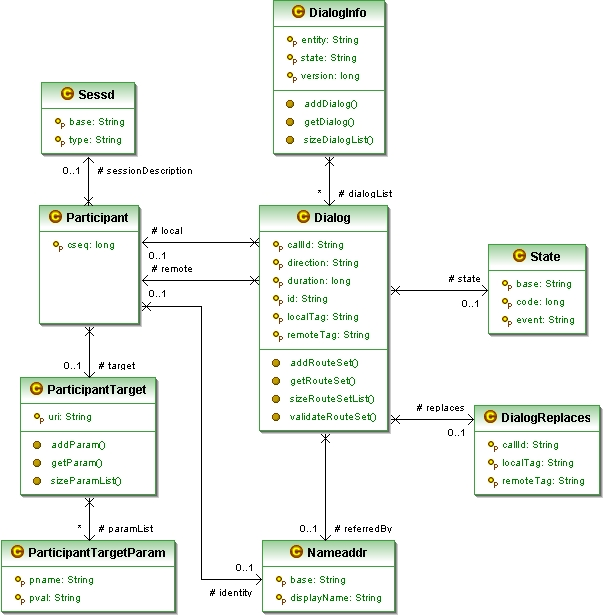
\includegraphics{dialoginfo.jpg}}
\caption{org.sipfoundry.dialoginfo Class Diagram}
\label{dialoginfoDiagram}
\end{figure}

To illustrate this in practice, the code snippet in Listing \ref{dialoginfoCode} shows the creation
of a partial \emph{dialog-info} which indicates that the second line
\emph{(x-line-id=1)} of extension 201 has gone off-hook.  Listing \ref{dialoginfoXML} then shows the corresponding XML code
that JiBX produces when the \emph{dialogInfo} object is marshaled out.  The process of unmarshaling
would be the inverse, where JiBX is given an XML document to unmarshal which would then result in an
instance of DialogInfo, along with zero or more Dialog instances, being created.

\lstset{emph={dialogInfo,dialog,state,local,target,param},
emphstyle=\color[RGB]{0,0,192}}
\begin{lstlisting}[float,captionpos=b,caption=Creation of basic dialog-info,label=dialoginfoCode]
DialogInfo dialogInfo = new DialogInfo();
dialogInfo.setVersion(47L);
dialogInfo.setState("partial");
dialogInfo.setEntity("sip:201@acme.com");

Dialog dialog = new Dialog();
dialog.setDirection("initiator");
dialog.setId("id12345678");
dialogInfo.addDialog(dialog);

State state = new State();
state.setBase("trying");
dialog.setState(state);

Participant local = new Participant();
dialog.setLocal(local);

ParticipantTarget target = new ParticipantTarget();
target.setUri("sip:201@acme.com");
local.setTarget(target);

ParticipantTargetParam param = new ParticipantTargetParam();
param.setPname("x-line-id");
param.setPval("1");
target.addParam(param);

dialogInfoMarshaler.marshalDocument(dialogInfo, "UTF-8", null, writer);
\end{lstlisting}

\lstset{emph={xml,dialog,info,dialog,state,local,target,param},
emphstyle=\color[RGB]{63,127,95}\bfseries,
emph={[2]version,encoding,xmlns,entity,id,direction,pname,uri,pname,pval},
emphstyle={[2]\color[RGB]{127,0,85}\bfseries}}
\begin{lstlisting}[float,captionpos=b,caption=Results of marshaled DialogInfo instance,label=dialoginfoXML]
<?xml version="1.0" encoding="UTF-8"?>
<dialog-info xmlns="urn:ietf:params:xml:ns:dialog-info"
                    version="47" state="partial" entity="sip:201@acme.com">
  <dialog id="id12345678" direction="initiator">
    <state>trying</state>
    <local>
      <target uri="sip:201@acme.com">
        <param pname="x-line-id" pval="1"/>
      </target>
    </local>
  </dialog>
</dialog-info>
\end{lstlisting}

\subsection{Appearance Group}
The Appearance Group component is where the actual business logic for the various \PAA supported
features such as Bridged Line Appearance (BLA) and Busy Lamp Field (BLF) reside.  The core
functionality of the Appearance Group component is to manage, aggregate and publish state
information of a collection of Appearance objects.  In the case of BLF, the collection could also
include other BLA Appearance Group objects.  The first phase will only include BLA business logic.

\subsubsection{Subscription Server}
The primary purpose of the Appearance Group component is to publish state information.  To that end,
the component will maintain a subscription server which can accept and service subscriptions
specific to the particular feature being supported.  For example, if the Appearance Group is of the
type BLA, then the subscription events will be of type \bold{dialog;ma}.  Also, in the case of a BLA
Appearance Group, the Subscription Server will attempt to skew the offered subscription expiration
time so as to have the expiration coincide with the underlying Appearance objects subscriptions. 
The goal is to have both sets of subscriptions expire at approximately the same time.

\subsubsection{Bridged Line Appearance Service}
In the first phase of this project, the Appearance Group component will be supporting a Bridged Line
Appearance (BLA) service per \emph{draft-anil-sipping-bla-03} and \emph{draft-anil-sipping-bla-04}. 
BLA, also referred to as Multiple Line Appearance, is an emulation of the traditional multi-line
keyed system.  The basic concept is for multiple stations to be able to share the same set of
lines/extensions.  A call arriving on one of the these lines will then ring on every station which
shares it. Once answered by one of the stations, the call can later be placed on hold and picked up
by any other station which shares that line.  The state of each one of the shared lines, either
idle, ringing, active or on-hold, is also displayed visually on each one of the associated stations.
 The traditional operational behavior of \emph{one call per line} or \emph{line seizure} is also
emulated.

\subsubsection{Appearance Number Allocation}
In the case where stations are provisioned with more than one appearance of a shared line, it then
becomes necessary to ensure constant allocation across stations.  For example, if a group of
stations are each provisioned with two appearances of extension 201, when a call arrives on 201,
each station needs to ring on the same appearance. If all stations are idle prior to the call
arriving, then the first appearance of each station will ring.  If, on the other hand, one of the
stations has gone off-hook on the first appearance, then the incoming call will ring on its second
appearance, while the other stations will ring on their first appearance.

To solve this problem, the standards call for the implementation to include a centralized appearance
number allocation mechanism.  This allocation mechanism would typically work in conjunction with the
systems forking proxy to add additional number allocation information to the outbound INVITE's via
the \emph{Alert-Info: appearance=n} header field.  In the above example, the \PAA would have known
that one of the stations had gone off-hook on the first line appearance.  The outbound INVITE's
generated by the incoming call would then have contained an \emph{Alert-Info: appearance=1} which
would direct the receiving stations to ring the call on their second appearance.

Note: \emph{It might be concluded that there could be a possible glare condition where the station
goes off-hook on line 1 at the same the incoming call arrives, resulting in the call being assigned
to that line.  Technically this condition cannot occur due to the fact that a station cannot truly
go off-hook until the \PAA has sent back positive acknowledgment.  This is referred to as ``line
seizure".}

Do to the inherent complexities associated with this feature, it will be necessary to defer this
feature until phase two of the project.  The result is that for the initial release, there will be a
limitation where a station will only be able to support a single appearance of a shared line.  It
will still be possible to support the intended work flow by employing hunt groups consisting of
shared lines.

\subsection{Appearance Manager}
The Appearance Manager component functions as the central location service for the \PAA by
maintaining mappings to all of the Appearance and Appearance Group instances.  Based upon
provisioning information, it works in conjunction with the Dependency Injector to instantiate the
required Appearance Group and Appearance instances.  Once instantiated, it then serves as the router
and context manager for all messaging and inbound signaling.

\subsection{Subscription Scheduler}
As stated earlier in this document, it is critical that the traffic associated with subscriptions be
kept as flat as possible, avoiding large bursts that could result in catastrophic congestion
failures.  Fortunately the majority of subscriptions that the \PAA deals with are either initiated
by the server or are as a direct response to subscriptions initiated by the server.  This fact
allows the server to have a great deal of influence on the timing and frequency of the
subscriptions.  For unsolicited subscriptions, such as what might be generated by another PBX
service such as a Call Pickup Server, there number will be relatively small and therefore not
considered to be an issue.

Most, if not all subscriptions initiated by the \PAA are done so in response to receiving a
notification registration event indicating that an appearance has gone into service.  In response to
this notification, the associated Appearance objects Subscription Client will need to subscribe for
dialog events.  If the target appearance is a shared line appearance, then it will also, in response
to receiving and accepting the subscription, initiate a subscription back to the \PAA.  The key to
controlling the rhythm of these subscriptions and their subsequent renewals is not to initiate the
sequence as soon as the registration notification is received.  Instead, queue the initiating
subscription requests and schedule there delivery over time.

The Subscription Scheduler is the component that is responsible for the operation of queuing and
scheduling the delivery of appearance dialog state subscriptions.  The basic concept is to maintain
a circular queue of buckets. Each bucket holds a set number of Subscription Client references. 
Figure \ref{ScheduleQueue} illustrates a Subscription Scheduler queue that consists of 8 buckets,
each with a capacity of 7.  This particular configuration, kept simple for illustration purposes,
thus has the capacity of handling a maximum of 56 appearances.  The number and depth of buckets will
be tunable and set to correspond to each deployments expected maximum capacity.  For example, to
handle a maximum of 300 appearances, the queue might be configured with 30 buckets each with a
capacity of 10.

\begin{figure}[ht] \centering
\scalebox{0.80}{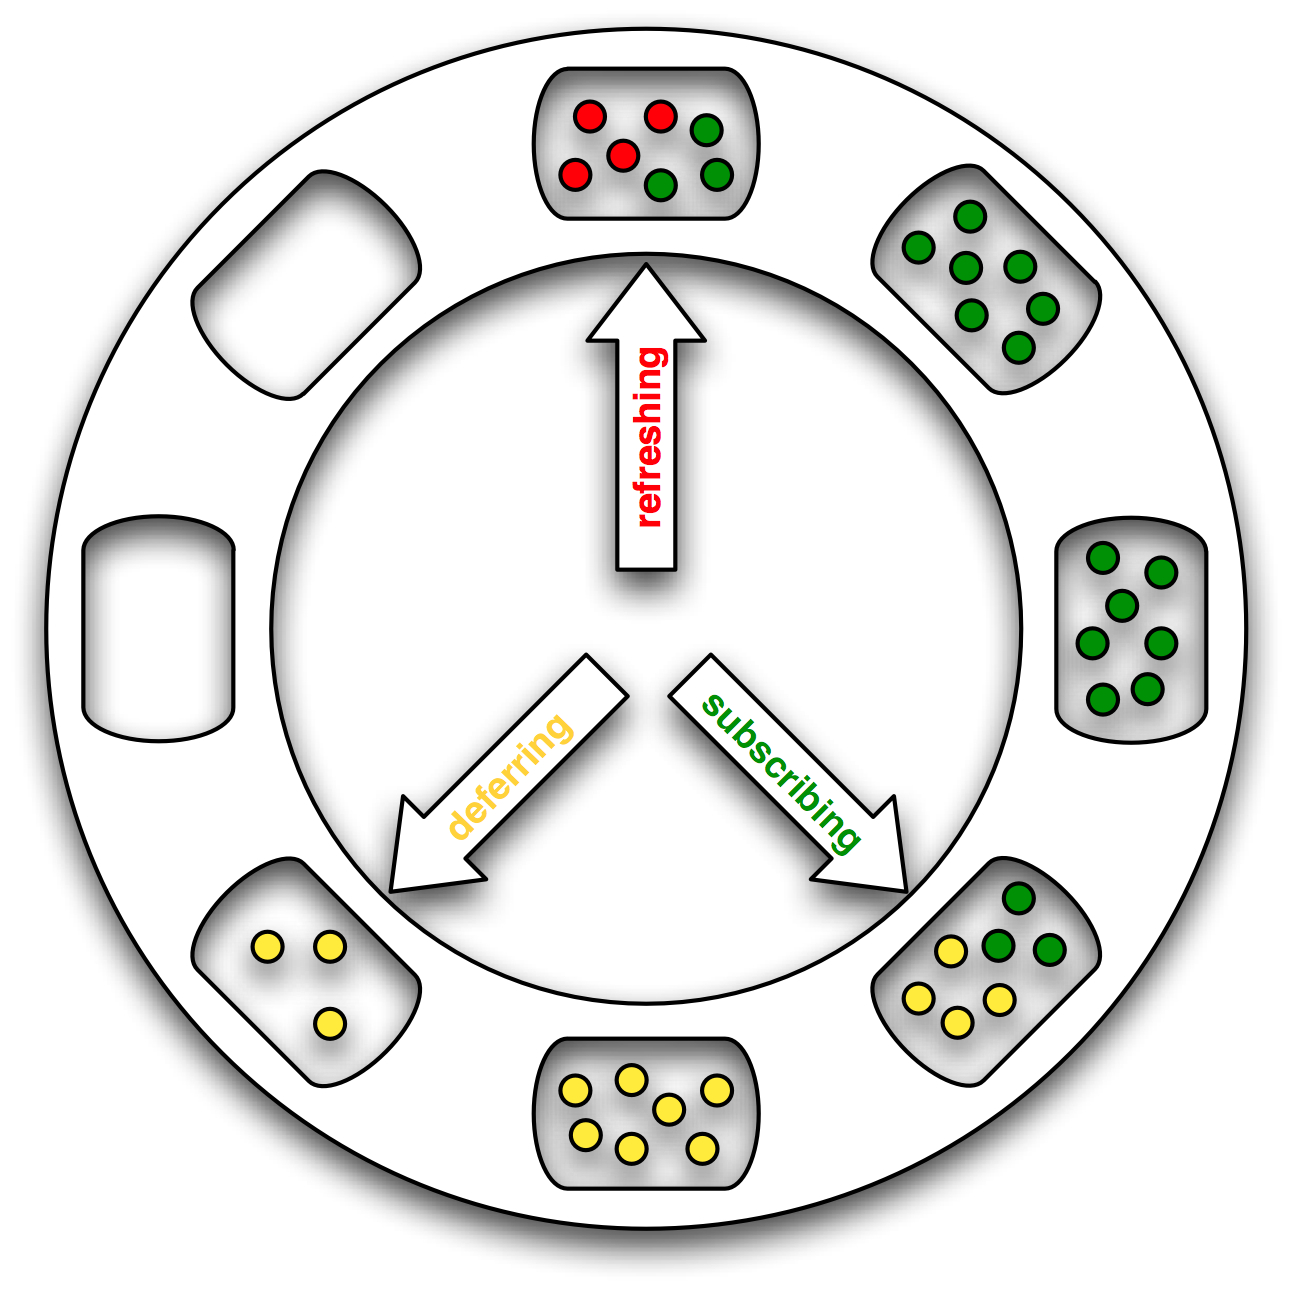
\includegraphics{scheduler.jpg}}
\caption{Subscription Scheduling Queue}
\label{ScheduleQueue}
\end{figure}

The queue operates three different indices's.  The first being the \yt{\bold{deferring}} index. 
This index begins at the first bucket, all of which are empty at start-up.  As Appearance objects,
via their Subscription Clients, begin initiating subscription requests, they are queued into the
indexed bucket.  Once the bucket is full, the index advances to the next bucket.  If there is a
misconfiguration and the number of subscription requests exceeds the queues capacity, a non-fatal
error will be reported and the additional requests will be distributed over the available buckets.

Over time, previously active subscriptions will become invalid and removed from their holding
bucket.  Later, new subscriptions will be made and placed in the bucket indexed by the
\yt{\bold{deferring}} index.  As this process repeats over time, the index will eventually wrap. 
When this occurs, the index will skip ahead to the first bucket that is not full.  If all are full,
it will fall back to the overflow mode.

Next is the \gt{\bold{subscribing}} index.  This index begins at the same bucket as the
\yt{\bold{deferring}} index.  All outstanding subscription requests that are in the bucket pointed
to by this index will be immediately dispatched.  Once there are no more outstanding requests and
the bucket is full, the index can prepare to advance to the next bucket.  If the bucket is not full,
the index will remain in place and as new requests are added, they will be immediately dispatched. 
One small difference is that the subscription expiration time for these stragglers will be adjusted
down so that they expire at approximately the same time as the others in the group.

Note: \emph{The expiration time of these subscriptions are used by the Subscription Server to adjust
the expiration time of any corresponding subscription requests that are received.  By doing this,
both sets of subscriptions should expire at approximately the same time.}

With the bucket full, the index can advance, but not immediately.  Instead, a delay is applied. 
This delay is very important as it sets the maximum rate in which subscriptions will be serviced. 
This will be a tunable parameter based upon the sizing of the deployment and the capacity of the
underlying hardware but will initially default to 5 seconds.

Finally there is the \rt{\bold{refreshing}} index.  This index begins at the same bucket as the
other two indexes.  Once one or more subscriptions become active within the bucket that it is
pointing to, it will set a timer corresponding to the most immediate expiration time of all active
subscriptions minus a subscription refresh acceleration time.  When the timer expires, all of the
active subscriptions in the bucket will be renewed.  The index will then advance to the next bucket
and repeat the process.  This continues for the life of the server and is the driving mechanism for
maintaining subscriptions to UA appearances.

\subsection{Dependency Injector}
The \PAA is architected around an Inversion of Control (IoC) pattern.  To
support this, the Google Guice (\emph{pronounced ``juice"}) IoC framework will
be employed as the dependency injection mechanism.  \emph{More research still needs to be done before it is completely understood how this will all come together.}

\subsection{Registration Notification Client}
Details are TBD.

\subsection{Appearance State Publisher}
The Appearance State Publisher provides a centralized source of state and dialog information for
external services and applications.  It will support a \emph{subscribe / publish} model utilizing
both SIP dialog-events and Java Messaging Service (JMS) running over XML-RPC.  A SIP based
application such as the Resource List Server (RLS) would utilize the dialog-event method and a WEB
based application such as the Attendant Console would utilize JMS.

Additional design details will be covered in a future version of this document.

\subsection{Provisioning}
Details are TBD.

\section{External Dependencies}
External dependencies are still being identified.  At this point, there are several that are at
least known to require further understanding.  These are:

\begin{itemize}
  \item Registrar Server registration notification events
  \item UA's operating over TCP / TLS transport
  \item Configuration Server support for shared line provisioning
\end{itemize}

\section{Design Verification}
Key to any project is the design verification.  For this project, three
distinct verification strategies are employed.

\subsection{Unit Testing}
One of the motivations for utilizing IoC is that it allows for easier development of
compartmentalized unit tests.  It is intended that this project take full advantage of this and the
development of each component will not be considered complete unless it includes at least a minimum
set of unit tests.

\subsection{Load Testing}
It is critical to fully understand how the server behaves under various loads and to determine what
the upper limits are.  The problem is how to generate these loads.  Using actual phones to generate
load is only practical up to several hundred lines.  Beyond that, it then becomes necessary to rely
on some type of load simulation.  A separate effort will need to be initiated to address this issue.

\subsection{Functional Testing}
A functional test plan will need to be assembled for use, both by the developers and by QA.  Details
are TBD.

\section{Clustering}
Due to the high degree of network traffic associated with \PAA functionality, it might not be
desirable to rely on a centralized server when dealing with a branch office deployments.  Therefore
it will be necessary to support a configuration where multiple \PAA servers are employed.  In this
configuration, appearances would be serviced by specific \PAA servers so as to minimize long hauling
of state traffic.  For state information which must span multiple sites, the servers servicing the
corresponding sites will manage the task of exchanging / synchronizing the appearance state
information and proxying to the subscribing appearances.

Additional Clustering design details will be covered in a future version of this document.

\section{High Availability}
In order for services which rely on timely information from the \PAA to be fault tolerant, it is
necessary for the server to support some form of high availability.  The approach that will be taken
builds upon the clustering support in the form of a warm standby server.  The active server will be
paired with a second server which operates passively in a standby state.  The active server will
then, in real time, synchronize both provisioning and appearance state information with the standby
server.  Subscriptions will not be replicated on the standby server.

In the case of a fail-over, the standby server will immediately begin to establish its own
subscriptions with the appearances.  In response, the appearances will establish new subscriptions
with the standby server.  Since the appearance state information has been preserved, the server will
be able to immediately publish accurate state information to the appearances, resulting in little or
no loss of service.

The idea is that the Subscription Scheduler on the standby server will be primed with all of the
required subscription requests, kept in sync via a TBD mechanism. Once put into service, the
\gt{\bold{subscribing}} index will begin working its way through the queue, dispatching the
``standby'' subscriptions.  As stated earlier, the rate in which the \gt{\bold{subscribing}} index
works its way through the queue is tunable.  So depending on how aggressively configured, it could
take from several seconds to several minutes to completely recover.

Additional High Availability design details will be covered in a future version of this document.

\section{References}
\subsection{Standards Documents}
\begin{enumerate}
  \item Soroushnejad, M., Venkataramanan, V., Pepper, P., Kumar, A., Johnston, A.,\\
  ``\bold{Implementing Multiple Line Appearances using the Session
  Initiation Protocol (SIP)}'', draft-anil-sipping-bla-03 (work in progress), June 2006
  \item Soroushnejad, M., Venkataramanan, V., Pepper, P., Kumar, A., Johnston, A.,\\
  ``\bold{Implementing Multiple Line Appearances using the Session
  Initiation Protocol (SIP)}'', draft-anil-sipping-bla-04 (work in progress), March 2007
  \item Rosenberg, J., Schulzrinne, H., and R. Mahy, ``\bold{An INVITE-Initiated
  Dialog Event Package for the Session Initiation Protocol (SIP)}", RFC 4235,
  November 2005.
  \item Roach, A. B., ``\bold{Session Initiation Protocol (SIP)-Specific
  Event Notification}", RFC 3265, November 2002.
  \item Johnston, A., Soroushnejad, M., Venkataramanan, V., Pepper, P., Kumar, A.,\\
  ``\bold{Requirements and Implementation Options for the Multiple Line
  Appearance Feature using the Session Initiation Protocol (SIP)}'',
  draft-johnston-bliss-mla-req-00 (work in progress), February 2007
\end{enumerate}

\subsection{Third Party Frameworks}
\begin{enumerate}
  \item \bold{jain-sip}, Java API for SIP Signaling (JSR-32),
  http://jain-sip.dev.java.net
  \item \bold{JiBX}, Framework for Binding XML Data to Java Objects, http://jibx.sourceforge.net
  \item \bold{XMLBeans}, Framework for Binding XML Data to Java Objects,\\
  http://xmlbeans.apache.org
  \item \bold{Guice}, Ultra-lightweight dependency injection container,
  http://code.google.com/p/google-guice
  \item \bold{eXist}, Open Source Native XML Database, http://exist.sourceforge.net
  \item \bold{mom4j}, Lightweight Java Message Service (JMS) Implementation,\\
  http://mom4j.sourceforge.net
  \item \bold{JEnable}, Source Configuration Program for Java,\\
  http://www.sosnoski.com/opensrc/jenable
\end{enumerate}

\end{document}               % End of document.
